% !TEX root = ../OT4ML.tex

\section{Generalized OT Problems}
\label{sec-generalized-ot-problems}

The second family changes the optimization problem rather than only the ground distance. Barycenters average several measures, multi-marginal OT couples many measures at once, inverse OT learns the cost from observed transport, and weak OT allows randomized conditional responses. These formulations remain close to Kantorovich linear programming, but the object being optimized is richer than a single two-marginal coupling.

\subsection{OT Barycenters}
\label{sec-barycenters}

Barycenters ask how to average probability measures rather than points. This subsection explains the variational definition, the special closed forms in one dimension and for Gaussians, and the entropic algorithms used in practice.

\paragraph{Fr\'echet means.}

For discrete input histograms $\{\b_s\}_{s=1}^S$, with $\b_s \in \simplex_{n_s}$, and weights $\la \in \simplex_S$, a Wasserstein barycenter can be computed by minimizing
\eql{\label{eq-wass-discr}
	\umin{\a \in \simplex_n} \sum_{s=1}^S \la_s \MKD_{\C_s}(\a,\b_s),
}
where the cost matrices $\C_s \in \RR^{n \times n_s}$ are prescribed.

This barycenter problem was originally introduced by~\cite{Carlier_wasserstein_barycenter} following earlier ideas of~\cite{carlierekelandmatching}. For the quadratic cost on $\X=\RR^d$, their theory gives existence and uniqueness when at least one input measure is absolutely continuous, and more generally under hypotheses ensuring that the relevant optimal maps are well defined. Discrete existence, consistency and fixed-point constructions are further studied in~\cite{anderes2016discrete,alvarez2016fixed,leGouic2016existence}.

Given a set of input measures $(\be_s)_s$ defined on some space $\X$, the barycenter problem becomes
\eql{\label{eq-barycenter-generic}
	\umin{\al \in \Mm_+^1(\X)} \sum_{s=1}^S \la_s \MK_{\c}(\al,\be_s).
}
\begin{rem}[Two measures give a Wasserstein geodesic]
	For $S=2$, $c(x,y)=\norm{x-y}^2$ and weights $(1-t,t)$, the barycenter is the point at time $t$ on the Wasserstein geodesic between $\beta_0$ and $\beta_1$. If $T$ is the Brenier map from $\beta_0$ to $\beta_1$, this barycenter is $((1-t)\Id+tT)_\sharp\beta_0$, the McCann interpolation detailed in Section~\ref{sec-geodesic-convexity}. If no Monge map is available, the same construction uses an optimal coupling $\pi$ and the interpolation map $(x,y)\mapsto(1-t)x+ty$, giving $((1-t)x+ty)_\sharp\pi$.
\end{rem}
\begin{example}[Dirac inputs]
	Problem~\eqref{eq-barycenter-generic} generalizes the computation of barycenters of points $(x_s)_{s=1}^S \in \X^S$ to arbitrary measures. Indeed, if $\be_s=\de_{x_s}$ is a single Dirac mass, then a solution to~\eqref{eq-barycenter-generic} is $\de_{x^\star}$ where $x^\star$ is a Fr\'echet mean of the points $(x_s)_s$.
\end{example}

\begin{figure}[ht]
\centering
\begin{tabular}{@{}cc@{}}
\small one-dimensional quantile barycenters &
\small two-dimensional shape barycenters \\[-.15em]

\includegraphics[width=.42\linewidth]{figures/barycenters-four-shapes/quantile-grid.pdf} &

\includegraphics[width=.42\linewidth]{figures/barycenters-four-shapes/shape-grid.pdf}
\end{tabular}
\caption{Wasserstein barycenter grids for four corner measures. The left panel uses the one-dimensional formula $Q_{u,v}=\sum_{i,j}\lambda_{ij}(u,v)Q_{ij}$ and displays the densities reconstructed from the averaged quantiles. The right panel uses four deformation maps from a common reference cloud to simple shapes and averages these maps with the same bilinear weights, which is the discrete Monge analogue of a barycentric map. Colors interpolate between the four corners.}
\label{fig:barycenters-four-shapes}
\end{figure}

\begin{rem}[Mean of a quadratic barycenter]
	For $c(x,y)=\norm{x-y}^2$, the mean of the barycenter $\al^\star$ is necessarily the barycenter of the means,
	\eq{
			\int_\Xx x \d\al^\star(x) = \sum_s \la_s \int_\Xx x \d\be_s(x).
	}
	Indeed, the squared Wasserstein distance decomposes into a squared distance between means plus a centered Wasserstein term. Minimizing the resulting quadratic function of the barycenter mean gives the displayed identity. If the input measures have compact support, the usual multi-marginal barycentric construction also gives a barycenter supported in the convex hull of the input supports.
\end{rem}


%%%%%%%%%%%%%%%%%%%%%%%%%%%%%%%%%%%%%%%%%%%%%%%%%%%%%%%%%%%%%%%%%%%%%%%%%%%
\paragraph{Gaussian Case}

Gaussian barycenters show that the same separation as in the Gaussian Wasserstein formula~\eqref{eq-dist-gauss} persists: means average linearly, while covariances average according to the Bures--Wasserstein geometry.

\begin{rem}[Gaussian barycenters]
	The barycenter of Gaussian measures is Gaussian. In one dimension, it is obtained by averaging the means and the standard deviations, so the barycenter variance is the square of this averaged standard deviation. In higher dimensions, the covariance $\cov$ minimizes the Bures objective
	\[
		\cov \mapsto \sum_s \la_s \Bb(\cov,\cov_s)^2,
	\]
	and equivalently solves the fixed-point equation
	\[
		\cov =
		\sum_s \la_s
		\pa{\cov^{1/2}\cov_s\cov^{1/2}}^{1/2}.
	\]
	This is the covariance analogue of the usual Euclidean barycenter equation: the mean part averages linearly, while the covariance part averages through the Bures--Wasserstein geometry~\cite{alvarez2016fixed,bhatia2018bures}.
\end{rem}

\begin{figure}[ht]
\centering
\begin{tabular}{@{}cc@{}}
\small moderate anisotropy &
\small strong anisotropy \\[-.15em]
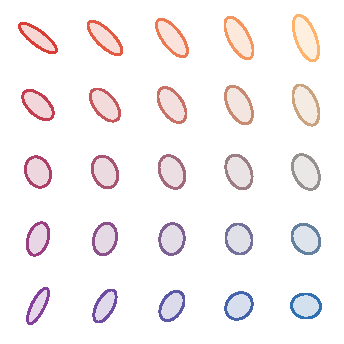
\includegraphics[width=.35\linewidth]{figures/barycenters-gaussian-covariances/moderate-grid.pdf} &
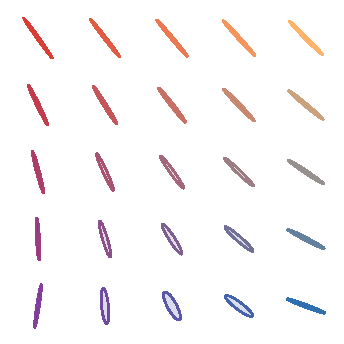
\includegraphics[width=.35\linewidth]{figures/barycenters-gaussian-covariances/anisotropic-grid.pdf}
\end{tabular}
\caption{Bures--Wasserstein barycenters of centered Gaussian covariance matrices. Each panel shows a $5\times5$ grid of barycenter ellipses for four corner covariances, without separate input panels: the corner ellipses are the four input covariances themselves. The right grid uses more anisotropic inputs, making the nonlinear rotation and scaling of covariance barycenters more visible.}
\label{fig:barycenters-gaussian-covariances}
\end{figure}


\begin{cor}[Gaussian and discrete barycenters]\label{cor-gaussian-discrete-barycenters}
		Quadratic Wasserstein barycenters of Gaussian measures are Gaussian. If the input measures are discrete, then there exists a barycenter supported on the set of weighted averages $\sum_s\la_s x_{s,i_s}$ of one support point from each input; in particular, if the $s$-th input has $n_s$ atoms, a barycenter exists with at most $\prod_s n_s$ atoms.
\end{cor}
\begin{proof}
		Let the input Gaussians have means $\mean_s$ and covariances $\cov_s$. For any candidate barycenter $\al$ with mean $\mean$ and covariance $\cov$, Gelbrich's inequality~\cite{gelbrich1990formula} gives
	\[
		\Wass_2^2(\al,\be_s)
		\geq
		\norm{\mean-\mean_s}^2+\Bb(\cov,\cov_s)^2,
	\]
	with equality for the Gaussian law with mean $\mean$ and covariance $\cov$. Therefore the barycenter objective is bounded below by a function depending only on $(\mean,\cov)$, and this lower bound is attained by the Gaussian measure with the minimizing mean and covariance. Hence at least one barycenter is Gaussian, and uniqueness in the usual nondegenerate setting gives the Gaussian barycenter mentioned above. For discrete inputs, the multi-marginal formulation uses the barycentric map
	\[
		B(x_1,\ldots,x_S)=\sum_s\lambda_s x_s.
	\]
	Any multi-marginal optimizer is supported on the finite product of the input supports, and $B$ maps this product to at most $\prod_s n_s$ points.
\end{proof}

\paragraph{Entropic regularization of multi-marginal.}

As in the two-marginal case, adding an entropic penalty with respect to the product measure $\al_1\otimes\cdots\otimes\al_S$ leads to scaling algorithms:
\[
		\inf_{\pi\in\Couplings(\al_1,\ldots,\al_S)}
		\int c\d\pi+\epsilon\KL(\pi|\al_1\otimes\cdots\otimes\al_S).
\]
The optimizer has the generalized Gibbs form
\[
	\d\pi^\star(x_1,\ldots,x_S)
	=
	\exp\!\left(\frac{\sum_s f_s(x_s)-c(x_1,\ldots,x_S)}{\epsilon}\right)
		\prod_s\d\al_s(x_s),
\]
and generalized Sinkhorn iterations alternately update one potential $f_s$ so that the $s$-th marginal is correct. The bottleneck is that a naive tensor representation has size $\prod_s n_s$ in the discrete case. Practical barycenter solvers therefore exploit separability of the cost, low-rank structure, convolutional kernels, or a fixed barycenter support.


%%%%%%%%%%%%%%%%%%%%%%%%%%%%%%%%%%%%%%%%%%%%%%%%%%%%%%%%%%%%%%%%%%%%%%%%%%%
%%%%%%%%%%%%%%%%%%%%%%%%%%%%%%%%%%%%%%%%%%%%%%%%%%%%%%%%%%%%%%%%%%%%%%%%%%%
%%%%%%%%%%%%%%%%%%%%%%%%%%%%%%%%%%%%%%%%%%%%%%%%%%%%%%%%%%%%%%%%%%%%%%%%%%%
\subsection{Metric learning and inverse OT}

This final subsection points to inverse problems where the ground cost itself is learned. Such problems are typically bilevel and non-convex, but OT provides useful gradients with respect to the cost.

%%%
\paragraph{Metric learning and derivatives of OT}

OT is convex with respect to the measure and concave with respect to the cost. Ground-metric learning was explicitly studied in~\cite{CuturiGroundMetric2014}, and it connects to the broader metric-learning literature~\cite{MAL-019,bellet2015metric}.

\begin{prop}[Derivative with respect to the cost]
	In the discrete setting, assume that the optimal coupling for $\MKD_\C(\a,\b)$ is unique and denote it by $\P^\star(\C)$. Then $\C \mapsto \MKD_\C(\a,\b)$ is differentiable at $\C$ and
	\[
		\nabla_\C \MKD_\C(\a,\b)=\P^\star(\C).
	\]
\end{prop}
\begin{proof}
	The value is the minimum of affine functions of $\C$,
	\[
		\MKD_\C(\a,\b)=\min_{\P\in\CouplingsD(\a,\b)}\dotp{\C}{\P}.
	\]
	The envelope theorem, or equivalently Danskin's theorem, states that the subdifferential with respect to $\C$ is the convex hull of the optimal couplings. If the optimizer is unique, this subdifferential is the singleton $\{\P^\star(\C)\}$, hence the value is differentiable with the displayed gradient.
\end{proof}

Thus, if the cost is parameterized as $\C_\theta$, gradients of losses involving OT values are obtained by backpropagating through the inner product $\dotp{\P^\star(\C_\theta)}{\partial_\theta \C_\theta}$. The difficulty is not differentiating a solved OT problem, but learning a cost for which the resulting matching has the desired semantic behavior; this is a bilevel and usually non-convex optimization problem.

\begin{figure}[ht]
\centering
\begin{tabular}{@{}ccc@{}}
\small Euclidean cost & \small moderate anisotropy & \small strong anisotropy \\[-.15em]

\includegraphics[width=.30\linewidth]{figures/metric-learning-cost-deformation/euclidean.pdf} &

\includegraphics[width=.30\linewidth]{figures/metric-learning-cost-deformation/moderate.pdf} &

\includegraphics[width=.30\linewidth]{figures/metric-learning-cost-deformation/strong.pdf}
\end{tabular}
\caption{Changing the ground metric changes the optimal coupling. The same red and blue empirical measures are matched with $c_A(x,y)=(x-y)^\top A(x-y)$ for the Euclidean metric and two increasingly anisotropic Mahalanobis metrics. The small gray ellipse shows the unit ball of the metric: directions in which the ellipse is elongated are cheaper, and this deforms the transport segments selected by the OT plan.}
\label{fig:metric-learning-cost-deformation}
\end{figure}

%%%
\paragraph{Inverse Optimal Transport}

Inverse OT asks for a ground cost that explains observed matchings or flows as optimal transport plans. In its most direct form, one observes a plan $\widehat\pi$ with marginals $(\alpha,\beta)$ and seeks a cost $c$ such that $\widehat\pi$ is optimal for
\[
	\inf_{\pi\in\Couplings(\alpha,\beta)}\int c(x,y)\d\pi(x,y).
\]
This is ill-posed without structure: adding potentials $u(x)+v(y)$ to a cost does not change the set of optimal couplings, and many costs can rationalize the same sparse plan.

A useful statistical methodology is to measure the suboptimality of the observed plan through a Fenchel--Young loss. Write the score as $s=-c$ and define the convex regularized prediction value
\[
	G_\epsilon(s)=
	\sup_{\pi\in\Couplings(\alpha,\beta)}
	\int s\d\pi-\epsilon\KL(\pi|\alpha\otimes\beta).
\]
The Fenchel--Young loss
\[
	\mathcal L_\epsilon(c;\widehat\pi)
	=
	G_\epsilon(-c)+G_\epsilon^*(\widehat\pi)+\int c\d\widehat\pi
\]
is nonnegative by Fenchel's inequality and vanishes exactly when $\widehat\pi\in\partial G_\epsilon(-c)$, i.e. when $\widehat\pi$ satisfies the regularized optimality conditions for $c$. Sharpened Fenchel--Young losses for inverse problems over measures and inverse entropic/unbalanced OT are developed in~\cite{andrade2025sharpened}; curvature and identifiability of inverse OT with respect to the cost are studied in~\cite{peyre2026curvature}. Entropic regularization is important here because it makes the forward map smoother and provides gradients with respect to $c$, at the price of a bias that must be controlled statistically.

In practice, one restricts the cost to a finite-dimensional model class, often affine:
\[
	C_\theta=\sum_{r=1}^R \theta_r C^{(r)},
	\qquad \theta\in\Theta,
\]
where $\Theta$ is convex and the matrices $C^{(r)}$ encode features, graph distances or a Mahalanobis parameterization. This viewpoint appears in low-rank and sparse inverse OT models~\cite{dupuy2016estimating,andrade2024sparsistency} and in convex formulations for learning OT costs from observed plans~\cite{ma2020learning,peyre2026curvature}.

\begin{prop}[Convex dual-gap formulation of inverse OT]\label{prop-inverse-ot-convex}
	Let $\widehat P\in\CouplingsD(\a,\b)$ be an observed coupling and let $C_\theta$ depend affinely on $\theta\in\Theta$, where $\Theta$ is convex. The condition that $\widehat P$ is optimal for the cost $C_\theta$ is equivalent to the existence of dual potentials $(f,g)$ such that
	\[
		f_i+g_j\leq (C_\theta)_{i,j}
		\qandq
		\sum_{i,j}\widehat P_{i,j}\big((C_\theta)_{i,j}-f_i-g_j\big)=0.
	\]
	Consequently, for a convex regularizer $R$, the noisy inverse problem can be relaxed as the convex program
	\eql{\label{eq-inverse-ot-convex}
		\umin{\theta\in\Theta,f,g}
		R(\theta)+\lambda
		\sum_{i,j}\widehat P_{i,j}\big((C_\theta)_{i,j}-f_i-g_j\big)
		\quad\text{subject to}\quad
		f_i+g_j\leq (C_\theta)_{i,j}\quad\forall i,j.
	}
\end{prop}

\begin{proof}
	For a fixed cost $C_\theta$, Kantorovich duality gives
	\[
		\min_{P\in\CouplingsD(\a,\b)}\dotp{C_\theta}{P}
		=
		\max_{f_i+g_j\leq (C_\theta)_{i,j}}
		\dotp{f}{\a}+\dotp{g}{\b}.
	\]
	Since $\widehat P$ has marginals $(\a,\b)$, every dual feasible pair satisfies
	\[
		\dotp{C_\theta}{\widehat P}-\dotp{f}{\a}-\dotp{g}{\b}
		=
		\sum_{i,j}\widehat P_{i,j}\big((C_\theta)_{i,j}-f_i-g_j\big)
		\geq0.
	\]
	This nonnegative quantity is exactly the primal-dual gap of $\widehat P$. It vanishes if and only if $\widehat P$ reaches the dual value and is therefore optimal. If $C_\theta$ is affine and $\Theta$ and $R$ are convex, the constraints and objective in~\eqref{eq-inverse-ot-convex} are convex, proving the relaxation claim.
\end{proof}

The formulation~\eqref{eq-inverse-ot-convex} is useful because it avoids differentiating through a forward OT solver: it learns a cost by making the observed plan satisfy complementary slackness. In statistical settings, $\widehat P$ is only partially observed or noisy, so one adds sparsity, low-rank, smoothness or metric constraints to select a meaningful cost~\cite{dupuy2016estimating,andrade2024sparsistency}. For entropic OT, the optimality condition becomes smoother:
\[
	\widehat P_{i,j}\approx a_i b_j
	\exp\pa{\frac{f_i+g_j-(C_\theta)_{i,j}}{\epsilon}},
\]
which leads to likelihood-based or KL-based convex objectives when $C_\theta$ is affine, and connects inverse OT with generalized Sinkhorn iterations and transport-regularized inverse problems~\cite{karlsson2016generalized,ma2020learning}. Neural parameterizations of $C_\theta$ are more flexible but reintroduce non-convexity; the convex formulation above is the clean mathematical baseline.


%%%%%%%%%%%%%%%%%%%%%%%%%%%%%%%%%%%%%%%%%%%%%%%%%%%%%%%%%%%%%%%%%%%%%%%%%%%


%%%%%%%%%%%%%%%%%%%%%%%%%%%%%%%%%%%%%%%%%%%%%%%%%%%%%%%%%%%%%%%%%%%%%%%%%%%
%%%%%%%%%%%%%%%%%%%%%%%%%%%%%%%%%%%%%%%%%%%%%%%%%%%%%%%%%%%%%%%%%%%%%%%%%%%
%%%%%%%%%%%%%%%%%%%%%%%%%%%%%%%%%%%%%%%%%%%%%%%%%%%%%%%%%%%%%%%%%%%%%%%%%%%
\subsection{Weak Optimal Transport}
\label{sec-weak-ot}

Weak OT relaxes the cost so that it depends on the conditional distribution of destinations rather than only on pointwise pairs. It is useful when a source point is allowed to choose a randomized response and the model only penalizes some aggregate of that response, such as its conditional mean. The framework was introduced through general transport costs and weak transport inequalities in~\cite{gozlan2017kantorovich}; existence, duality and optimality conditions on Polish spaces are developed in~\cite{backhoff2019weak}.

Given $\pi\in\Couplings(\alpha,\beta)$, disintegrate it as $\pi(\d x,\d y)=\pi_x(\d y)\alpha(\d x)$. For a weak cost $C:\X\times\Pp(\Y)\to\RR\cup\{+\infty\}$, the weak OT value is
\begin{equation}\label{eq-weak-ot}
	\mathcal{W}_C(\alpha,\beta)
	\eqdef
	\inf_{\pi\in\Couplings(\alpha,\beta)}
	\int C(x,\pi_x)\d\alpha(x).
\end{equation}
The classical Kantorovich problem is recovered when $C(x,\nu)=\int c(x,y)\d\nu(y)$, because the objective then becomes $\int c(x,y)\d\pi(x,y)$. The genuinely weak behavior starts when $C$ is nonlinear in $\nu$.

\begin{prop}[Weak Kantorovich duality]\label{prop-weak-ot-duality}
	Assume that $\X,\Y$ are compact metric spaces and that $C(x,\nu)$ is lower semicontinuous, bounded from below and convex in $\nu$, with the standard qualification assumptions ensuring Fenchel--Rockafellar duality. For $g\in\Cc(\Y)$ define the weak $C$-transform
	\[
		g^C(x)
		\eqdef
		\inf_{\nu\in\Pp(\Y)}
		\left\{
			C(x,\nu)-\int g(y)\d\nu(y)
		\right\}.
	\]
	Then
	\[
		\mathcal{W}_C(\alpha,\beta)
		=
		\sup_{g\in\Cc(\Y)}
		\left\{
			\int g^C(x)\d\alpha(x)+\int g(y)\d\beta(y)
		\right\}.
	\]
	When $C(x,\nu)=\int c(x,y)\d\nu(y)$, this reduces to the usual Kantorovich dual with $g^C(x)=\inf_y(c(x,y)-g(y))$.
\end{prop}

\begin{proof}
	For any coupling $\pi$ and any $g\in\Cc(\Y)$, the definition of $g^C$ gives
	\[
		C(x,\pi_x)\geq g^C(x)+\int g(y)\d\pi_x(y).
	\]
	After integration with respect to $\alpha$, the second term becomes $\int g\d\beta$ because the second marginal of $\pi$ is $\beta$. This proves weak duality.

	For the reverse inequality, consider the convex minimization over probability kernels $x\mapsto\pi_x$ with the affine constraint $\int \pi_x\d\alpha(x)=\beta$. Fenchel--Rockafellar duality gives a continuous Lagrange multiplier $g$ for this marginal constraint. Minimizing the Lagrangian over each conditional law gives exactly the pointwise term $g^C(x)$, while the multiplier contributes $\int g\d\beta$. The compactness, lower semicontinuity, convexity and qualification assumptions ensure no duality gap. This is the weak-cost analogue of Proposition~\ref{prop-duality-discr}.
\end{proof}

\begin{prop}[Barycentric weak transport is weaker than $\Wass_2$]\label{prop-barycentric-weak-ot}
	Let $\alpha,\beta\in\Pp_2(\RR^d)$ and define
	\[
		C_{\mathrm{bar}}(x,\nu)
		=
		\norm{x-\int y\d\nu(y)}^2.
	\]
	Then
	\[
		\mathcal{W}_{C_{\mathrm{bar}}}(\alpha,\beta)
		\leq
		\Wass_2^2(\alpha,\beta).
	\]
\end{prop}

\begin{proof}
	Let $\pi$ be any coupling and disintegrate it as $\pi_x\alpha$. By Jensen's inequality,
	\[
		\norm{x-\int y\d\pi_x(y)}^2
		\leq
		\int\norm{x-y}^2\d\pi_x(y).
	\]
	Integrating in $x$ gives $\int C_{\mathrm{bar}}(x,\pi_x)\d\alpha(x)\leq\int\norm{x-y}^2\d\pi(x,y)$. Taking the infimum over $\pi$ proves the claim.
\end{proof}

\begin{figure}[ht]
\centering
\begin{tabular}{@{}cc@{}}
\small conditional coupling & \small barycentric projection \\[-.15em]
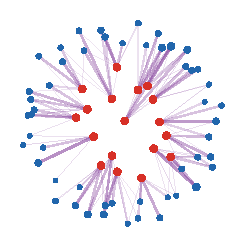
\includegraphics[width=.43\linewidth]{figures/weak-ot-barycentric-projection/conditional-coupling.pdf} &
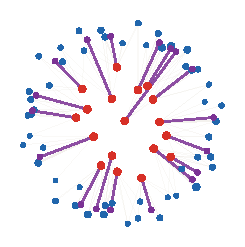
\includegraphics[width=.43\linewidth]{figures/weak-ot-barycentric-projection/barycentric-projection.pdf}
\end{tabular}
\caption{Weak barycentric transport on a small discrete coupling. The left panel shows the full conditional laws: each red source atom splits its mass among several blue target atoms, with segment thickness proportional to transported mass. The right panel collapses each conditional law $\pi_x$ to its barycenter $\bar y(x)=\int y\d\pi_x(y)$, shown in violet. The barycentric weak cost only sees the red-to-violet displacement, and therefore ignores the conditional spread around each barycenter.}
\label{fig:weak-ot-barycentric-projection}
\end{figure}

The barycentric cost is the canonical example to keep in mind: it only asks the conditional mean of $Y$ given $X=x$ to be close to $x$, and ignores the conditional variance. This connects weak OT with martingale transport, Strassen-type convex-order constraints, barycentric projections and learning problems where conditional averages are meaningful objects.
